\documentclass[12pt, titlepage]{article}
\usepackage{booktabs}
\usepackage{graphicx}
\usepackage{tabularx}
\usepackage{longtable}
\usepackage{hyperref}
\usepackage[section]{placeins}
\usepackage{makecell}
\usepackage{natbib}
\bibliographystyle{plain}
\graphicspath{ {./} }
\hypersetup{
    colorlinks,
    citecolor=black,
    filecolor=black,
    linkcolor=red,
    urlcolor=blue
}

\title{SE 3XA3: Test Report\\CraftMaster}

\author{Group 307, 3 Craftsmen
		\\ Hongqing Cao 400053625
		\\ Sida Wang 400072157
		\\ Weidong Yang 400065354
}

\date{\today}


\begin{document}

\maketitle

\pagenumbering{roman}
\tableofcontents
\listoftables
\listoffigures
\FloatBarrier
\begin{table}[bp]
\begin{tabularx}{\textwidth}{p{3cm}p{2cm}X}
\toprule {\bf Date} & {\bf Version} & {\bf Notes}\\
\midrule
April 2 & 1.0 & General content added\\
April 6 & 2.0 & Completed for Rev1\\
\bottomrule
\end{tabularx}
\caption{\bf Revision History}
\end{table}
\FloatBarrier
\newpage

\pagenumbering{arabic}

\section{Overview}
This document specifies the result of the testing specifications that are proposed in the \href{https://gitlab.cas.mcmaster.ca/wangs132/minecraft/-/blob/master/Doc/TestPlan/TestPlan.pdf}{\bf Test Plan} of CraftMaster. The format of this document follows the template provided by Dr.Bokhari and Thien Trandinh.
\subsection{Acronyms, Abbreviations, and Symbols}
\FloatBarrier
\begin{table}[hbp]
\begin{tabularx}{\textwidth}{p{3cm}X}
\toprule
\textbf{Abbreviation} & \textbf{Definition} \\
\midrule
SRS & Software Requirement Specification\\
OS & Operating System\\
GUI & Graphical User Interface\\
\bottomrule
\end{tabularx}
\caption{\textbf{Table of Abbreviations}} \label{Table}
\end{table}
\FloatBarrier
\FloatBarrier
\begin{table}[!htbp]

\begin{tabularx}{\textwidth}{p{3cm}X}
\toprule
\textbf{Term} & \textbf{Definition}\\
\midrule
Python & The programming language that is used for the developement of this project\\
Pyglet & A Python library for the design of graphical user interface\\
Pytest & A Python library and framework for unit testing\\
Sandbox Games & A type of game that allows player to create, modify, and destroy the environment\\
3D Game & A game in three dimensions\\

\bottomrule
\end{tabularx}
\caption{\textbf{Table of Definitions}} \label{Table}
\end{table}
\FloatBarrier


\newpage
\section{Functional Requirements Evaluation}


\FloatBarrier
\begin{center}
\begin{longtable}[!bpht]{|m{1.3cm}|m{2.3cm}|m{3.4cm}|m{3.4cm}|m{3.4cm}|m{1cm}|}\hline
\textbf{Test Case No.} & \textbf{Test Name} & \textbf{Initial State} & \textbf{Input} & \makecell[ml]{\textbf{Expected} \\\textbf{Output}}& \textbf{Pass or Fail}\\\hline

\textbf{TFR1} & \makecell[ml]{Test Game\\ Start} & \makecell[ml]{The software game\\ is installed and\\ ready to execute.} & \makecell[ml]{A cursor placement\\ on the game icon\\ and a double-click\\ on the left mouse\\ key.} & \makecell[ml]{The program opens\\ the GUI frame with\\ main menu\\ rendered.} & \textbf{Pass}\\\hline

\textbf{TFR2} & \makecell[ml]{Test Main\\ Menu and\\ Sub-Menus\\ directions} & \makecell[ml]{The GUI is opened\\ and the main menu\\ is rendered.} & \makecell[ml]{Mouse clicks on the\\ buttons on the\\ main menu that\\ direct to sub-menus\\ and buttons on the\\ sub-menus that\\ direct to the main\\ menu.} & \makecell[ml]{The program will\\ go to sub-menus\\ from the main\\ menu and go to the\\ main menu from\\ sub-menus.} & \textbf{Pass}\\\hline

\textbf{TFR3} & \makecell[ml]{Test New\\ Game} & \makecell[ml]{The GUI is opened\\ and the game menu\\ is rendered.} & \makecell[ml]{Mouse clicks on the\\ ``start new game"\\ button.} & \makecell[ml]{The program will\\ load a new game\\ scene, initialize the\\ character, and\\ place the crosshair\\ at the center of\\ the window.} & \textbf{Pass}\\\hline

\textbf{TFR4} & \makecell[ml]{Test Saved\\ Game} & \makecell[ml]{The GUI is opened\\ and the game menu\\ is rendered. There\\ is a saved game\\ scene.} & \makecell[ml]{A mouse clicks on\\ the "load game"\\ button and a\\ mouse clicks on a\\ game saving spot\\(Game One or\\ Game Two).} & \makecell[ml]{The program will\\ load a saved game\\ scene, initialize\\ the character, and\\ place the crosshair\\ at the center of\\ the window.} & \textbf{Pass}\\\hline

\textbf{TFR5} & \makecell[ml]{Test\\ Crosshair\\ Position\\ Stability} & \makecell[ml]{The software game\\ GUI is opened\\ and the crosshair\\ is placed at the\\ center of the GUI\\ window.} & \makecell[ml]{A sequence of\\ movements of\\ the character\\(controlled by\\ keyboard inputs)\\ followed by a\\ sequence of block\\ operations\\(controlled by\\ keyboard and\\ mouse inputs).} & \makecell[ml]{The crosshair\\ keeps in position\\ (center of GUI\\ window).} & \textbf{Pass}\\\hline

\textbf{TFR6} & \makecell[ml]{Test\\ Character\\ Direction} & \makecell[ml]{The software game\\ GUI is opened and\\ the game scene\\ and character are\\ loaded.} & \makecell[ml]{A movement of\\ the mouse.} & \makecell[ml]{The character\\ changes its view\\ direction.} & \textbf{Pass}\\\hline

\textbf{TFR7} & \makecell[ml]{Test Block\\ Outline} & \makecell[ml]{The software game\\ GUI is opened and\\ the game scene\\ and character are\\ loaded. A block is\\ near the character.} & \makecell[ml]{A movement of the\\ mouse to aim the\\ crosshair at the\\ block.} & \makecell[ml]{The GUI shows\\ the outline of the\\ block(indicating\\ the block is being\\ aimed at).} & \textbf{Pass}\\\hline

\textbf{TFR8} & \makecell[ml]{Test Block\\ Removal} & \makecell[ml]{The software game\\ GUI is opened and\\ the game scene\\ and character are\\ loaded. A block is\\ near the character\\ and the player has\\ already aimed the\\ crosshair at the\\ block.} & \makecell[ml]{A left-click on\\ the mouse.} & \makecell[ml]{The block is\\ being removed\\ from the window\\ and the program\\ plays a sound effect\\ to notify.} & \textbf{Pass}\\\hline

\textbf{TFR9} & \makecell[ml]{Test Block\\ Build} & \makecell[ml]{The software game\\ GUI is opened and\\ the game scene\\ and character are\\ loaded. A block is\\ near the character\\ and the player has\\ already aimed the\\ crosshair at the\\ block(the crosshair\\ could be pointed\\ to top, bottom, or\\ any side).} & \makecell[ml]{A right-click on\\ the mouse.} & \makecell[ml]{The new block is\\ being built at the\\ position that is\\ next to the surface\\ of \hspace{-0.5mm}the \hspace{-0.5mm}existing \hspace{-0.5mm}block\\ that the crosshair\\ was pointed to and\\ the program plays\\ a sound effect to\\ notify.} & \textbf{Pass}\\\hline

\textbf{TFR10} & \makecell[ml]{Test\\ Background\\ Music} & \makecell[ml]{The software game\\ is installed and\\ ready to execute.} & \makecell[ml]{A cursor placement\\ on the game icon\\ and a double-click\\ on the left mouse\\ key.} & \makecell[ml]{The program plays\\ the background\\ music of the game.} & \textbf{Pass}\\\hline

\textbf{TFR11} & \makecell[ml]{Test Marble\\ Block\\ Operations} & \makecell[ml]{A \hspace{-0.5mm}crosshair \hspace{-0.5mm}is \hspace{-0.5mm}placed\\ on a marble block.} & \makecell[ml]{A left-click on\\ the mouse.} & \makecell[ml]{The marble is\\ not removed.} & \textbf{Pass}\\\hline

\textbf{TFR12} & \makecell[ml]{Test\\ Day-Night\\ Mode} & \makecell[ml]{The GUI is at the\\ setting menu or at\\ the ESC menu.} & \makecell[ml]{A left-click on the\\ Day-Night Mode\\ switch.} & \makecell[ml]{The Day-Night\\ mode changes.} & \textbf{Pass}\\\hline

\textbf{TFR13} & \makecell[ml]{Test Game\\ Quit} & \makecell[ml]{The GUI is at the\\ main menu.} & \makecell[ml]{A left-click on\\``quit" button on\\ the main menu.} & \makecell[ml]{The program\\ terminates and\\ the GUI closes.} & \textbf{Pass}\\\hline

\textbf{TFR14} & \makecell[ml]{Test Game\\ Save} & \makecell[ml]{The GUI is at\\ ESC menu.} & \makecell[ml]{A \hspace{-0.5mm}left-click \hspace{-0.5mm}on \hspace{-0.5mm}game\\ saving and saving\\ spot selection\\ button.} & \makecell[ml]{The json file\\ appears in the\\ game folder.} & \textbf{Pass}\\\hline

\textbf{TFR15} & \makecell[ml]{Test ESC\\ menu to\\ Game menu} & \makecell[ml]{The GUI is at\\ ESC menu.} & \makecell[ml]{A \hspace{-0.5mm}left-click \hspace{-0.5mm}on \hspace{-0.5mm}game\\ saving and saving\\ spot selection\\ button.} & \makecell[ml]{The GUI returns\\ to the game menu.} & \textbf{Pass}\\\hline


\textbf{TFR16} & \makecell[ml]{Test\\ Forward\\ Movement} & \makecell[ml]{The software game\\ GUI is opened and\\ the game scene and\\ character are\\ loaded. The\\ character is free to\\ move forward(no\\ blocks are close to\\ and at the front of\\ the character).} & \makecell[ml]{A click on the\\ ``W" key on the\\ keyboard.} & \makecell[ml]{The character\\ moves forward.} & \textbf{Pass}\\\hline

\textbf{TFR17} & \makecell[ml]{Test Left\\ Movement} & \makecell[ml]{The software game\\ GUI is opened and\\ the game scene and\\ character are\\ loaded. The\\ character is free to\\ 
move to the left(no\\ blocks are close to\\ and on the left of\\ the character).} & \makecell[ml]{A click on the\\ ``A" key on the\\ keyboard.} & \makecell[ml]{The character\\ moves to the left.} & \textbf{Pass}\\\hline

\textbf{TFR18} & \makecell[ml]{Test\\ Backward\\ Movement} & \makecell[ml]{The software game\\ GUI is opened and\\ the game scene and\\ character are\\ loaded. The\\ character is free to\\ move backward(no\\ blocks are close to\\ and at the back of\\ the character).} & \makecell[ml]{A click on the\\ ``S" key on the\\ keyboard.} & \makecell[ml]{The character\\ moves backward.} & \textbf{Pass}\\\hline

\textbf{TFR19} & \makecell[ml]{Test Right\\ Movement} & \makecell[ml]{The software game\\ GUI is opened and\\ the game scene and\\ character are\\ loaded. The\\ character is free to\\ move to the right\\(no blocks are close\\ to and on the right\\ of the character).} & \makecell[ml]{A click on the\\ ``D" key on the\\ keyboard.} & \makecell[ml]{The character \\moves to the right.} & \textbf{Pass}\\\hline

\textbf{TFR20} & \makecell[ml]{Test Jump\\ Action} & \makecell[ml]{The software game\\ GUI is opened and\\ the game scene and\\ character are\\ loaded.} & \makecell[ml]{A click on the\\ space key on the\\ keyboard.} & \makecell[ml]{The character\\ jumps once.} & \textbf{Pass}\\\hline

\textbf{TFR21} & \makecell[ml]{Test\\ Flying Mode} & \makecell[ml]{The software game\\ GUI is opened and\\ the game scene and\\ character are\\ loaded.} & \makecell[ml]{A click on the tab\\ key, followed a\\ sequence of clicks\\ on the ``W" and\\ ``S" keys, and\\ followed by a click\\ on the tab key on\\ the keyboard.} & \makecell[ml]{The flying mode\\ is activated, the\\ character flies and\\ then the flying\\ mode is\\ deactivated.} & \textbf{Pass}\\\hline

\textbf{TFR22} & \makecell[ml]{Test Block\\ Type Change\\ - Brick} & \makecell[ml]{A block is near the\\ character and the\\ player has already\\ aimed the crosshair\\ at the block(the\\ crosshair could be\\ pointed to top,\\ bottom, or any\\ side).} & \makecell[ml]{A click on the ``1"\\ key on the\\ keyboard, followed\\ by a right-click on\\ the mouse.} & \makecell[ml]{A brick block\\ is built.} & \textbf{Pass}\\\hline

\textbf{TFR23} &  \makecell[ml]{Test Block\\ Type Change\\ - Grass} & \makecell[ml]{A block is near the\\ character and the\\ player has already\\ aimed the crosshair\\ at the block(the\\ crosshair could be\\ pointed to top,\\ bottom, or any\\ side).} & \makecell[ml]{A click on the ``2"\\ key on the\\ keyboard, followed\\ by a right-click on\\ the mouse.} & \makecell[ml]{A grass block\\ is built.} & \textbf{Pass}\\\hline

\textbf{TFR24} & \makecell[ml]{Test Block\\ Type Change\\ - Stone} & \makecell[ml]{A block is near the\\ character and the\\ player has already\\ aimed the crosshair\\ at the block(the\\ crosshair could be\\ pointed to top,\\ bottom, or any\\ side).} & \makecell[ml]{A click on the ``3"\\ key on the\\ keyboard, followed\\ by a right-click on\\ the mouse.} & \makecell[ml]{A stone block\\ is built.} & \textbf{Pass}\\\hline

\textbf{TFR25} & \makecell[ml]{Test ESC\\ menu Open} & \makecell[ml]{The software game\\ GUI is opened.} & \makecell[ml]{A click on the\\ ``ESC" key on the\\ keyboard.} & \makecell[ml]{The cursor is\\ released from the\\ GUI and the ESC\\ menu opens.} & \textbf{Pass}\\\hline

\textbf{TFR26} & \makecell[ml]{Test\\ Block-Through\\ Movement} & \makecell[ml]{The character is on\\ a position where\\ is surrounded by\\ blocks.} & \makecell[ml]{A sequence of\\ clicks on ``W",\\ ``A", ``S", ``D".} & \makecell[ml]{The character does\\ not move through\\ the surrounding\\ blocks.}& \textbf{Pass}\\\hline

\textbf{TFR27} & \makecell[ml]{Test Trivial\\ Keys} & \makecell[ml]{The GUI is loaded\\ with a game scene.} & \makecell[ml]{A sequence of\\ mouse clicks on\\ keys that are not\\ assigned with any\\ task, in this case\\ use `Z', `P', `0', `;',\\ `CTRL'.} & \makecell[ml]{The system does\\ nothing to respond\\ and also does not\\ crash.} & \textbf{Pass}\\\hline

\makecell[ml]{\textbf{TFR}\\\textbf{4.1}} & \makecell[ml]{Test Saved\\ Game\\ Exception} & \makecell[ml]{The GUI is opened\\ and the game\\ menu is rendered.\\ There is no saved\\ game scene.} & \makecell[ml]{A mouse clicks on\\ the ``load game”\\ button and a\\ mouse clicks on\\ a game saving spot\\ (Game One or\\ Game Two).} & \makecell[ml]{The buttons that\\ control the saving\\ spot selection are\\ not clickable and\\ the system will not\\ load a game scene.} & \textbf{Pass}\\\hline

\makecell[ml]{\textbf{TFR}\\\textbf{20.1}} & \makecell[ml]{Test Jump\\ Action Edge} & \makecell[ml]{The software game\\ GUI is opened and\\ the game scene and\\ character are\\ loaded. The\\ character is in a\\ narrow space.} & \makecell[ml]{A click on the\\ space key on the\\ keyboard.} & \makecell[ml]{The character does\\ not jump.} & \textbf{Pass}\\\hline

\makecell[ml]{\textbf{TFR}\\\textbf{7.1}} & \makecell[ml]{Test Block\\ Outline Edge} & \makecell[ml]{The software game\\ GUI is opened and\\ the game scene and\\ character are\\ loaded. Two\\ connected blocks are\\ near the character.} & \makecell[ml]{A movement of\\ the mouse to aim\\ the crosshair at\\ the middle of \\two blocks.} & \makecell[ml]{The GUI shows the\\ outline of the\\ block that is closer\\ to the crosshair.} & \textbf{Pass}\\\hline

\makecell[ml]{\textbf{TFR28}} & \makecell[ml]{Test Menu\\ Click\\ Exception} & \makecell[ml]{The software game\\ GUI is rendered\\ with any menu.} & \makecell[ml]{A sequence of\\ clicks on the empty\\ spaces on the menu.} & \makecell[ml]{The software game\\ does nothing to\\ respond and does\\ not crash.} & \textbf{Pass}\\\hline
\caption{\bf{Tests for Functional Requirements Result}}
\end{longtable}
\end{center}
\FloatBarrier



\section{Non-functional Requirements Evaluation}

\subsection{Appearance}
\begin{enumerate}

\item{\textbf{TNFR1 Test Look and Feel\\}}
Initial State: The game is installed and is given to a group of teenage players.

Expected Result: The group should be satisfied with the attractiveness and style of the game.

Result: The survey was given to three teenage family members of the testing team. The average of the survey result was above the expected average value.

Pass/Fail: Pass

Significance: The test result reflects that the software game product is attractive enough to teenage players.

\end{enumerate}
\subsection{Usability}
\begin{enumerate}

\item{\textbf{TNFR2: Test Game Difficulty \\}}
Initial State: The game is installed and is given to a group of random aged people to play.

Condition: The group should be able to play the game with no difficulty.

Result: The survey was given to ten family members of the testing team that are from different age groups. The average of the survey result was slightly above the expected average value.

Pass/Fail: Fail

Significance: The test result reflects that the software game product is slightly difficult for everyone to play. 

\item{\textbf{TNFR3: Test Learning Curve \\}}
Initial State: The game is installed and is given to a group of random aged people to play.

Condition: The group should be able to learn the game within a time between \textbf{LEARN\_MIN} to \textbf{LEARN\_MAX} minutes.

Result: The survey was given to ten family members of the testing team that are from different age groups. The average of the survey result was within the expected time period. However, some of the group members reported that it was difficult for them to learn the game within \textbf{LEARN\_MAX} minutes.

Pass/Fail: Pass

Significance: The test result reflects that the software game product is slightly difficult for everyone to learn. The feedback reflects that the it takes time for some individuals to get familiar with the menus and button.

\end{enumerate}
\subsection{Performance}
\begin{enumerate}
\item{\textbf{TNFR4: Test Speed\\}}
Initial State: The game is installed.

Condition: The software game should respond to game events in less than \textbf{RESPONSE} second for 99\% of the interrogations and no response should take longer than \textbf{FALSE\_RESPONSE} second.

Result: The response time of the software game passed the condition of the test case.

Pass/Fail: Pass

Significance: The test result reflects that the Python language and Pyglet provides sufficient execution speed for this software game.

\item{\textbf{TNFR5: Test Availability\\}}
Initial State: The game is installed.

Condition: The software game should allow access to the game at different times.

Result: All accesses to the game were successful.

Pass/Fail: Pass

Significance: The test result reflects that the availability of this software game is stable.

\item{\textbf{TNFR6: Test Reliability\\}}
Initial State: The game is installed.

Condition: The software game should run for five hours.

Result: The software game successfully ran for eight hours. By the end of the eight hours, the tester shut down the game.

Pass/Fail: Pass

Significance: The test result reflects that this software game is reliable.

\end{enumerate}	

\subsection{Operational and Environmental Aspects}
\begin{enumerate}
\item{\textbf{TNFR7: Test Adjacent System Effect\\}}\label{adjacent}
Initial State: The game is installed.

Condition: The software game should not produce any negative effects on adjacent systems.

Result: The tester monitored other programs' performance while running CraftMaster. Some of other programs such as Microsoft Teams experienced latency effect.

Pass/Fail: Fail

Significance: The test result reflects that this software game might produce negative effects on adjacent systems.
\end{enumerate}

\subsection{Maintainability and Support}
\begin{enumerate}
\item{\textbf{TNFR8: Test Adaptability\\}}
Initial State: The game is available to be downloaded from internet.

Condition: The software game should be easily downloaded, installed, and opened onto both Windows and Linux OS.

Result: The tester downloaded, installed and opened the game on both Windows and Linux OS.

Pass/Fail: Pass

Significance: The test result reflects that this software game is adaptable to both Windows and Linux OS.

\end{enumerate}

\subsection{Security}
\begin{enumerate}
\item{\textbf{TNFR9: Test Integrity\\}}
Initial State: The game is installed.

Condition: The software game should prevent low level threats.

Result: The tester created three threat test cases to intentionally abuse the software game. The software did not fail.

Pass/Fail: Pass

Significance: The test result reflects the software game is integrity is convinced to some extent.
\end{enumerate}

\subsection{Cultural Aspects}
\begin{enumerate}
\item{\textbf{TNFR10: Test Cultural Politeness\\}}
Initial State: The game is installed and is given to a group of people from different cultural groups to play.

Condition: The group should have satisfaction with the cultural politeness of the game.

Result: The survey was given to ten friends and family members of the testing team that are from China and Canada. The average of the survey result was above the expected value.

Pass/Fail: Pass

Significance: The test result reflects the software game is cultural polite.
\end{enumerate}

\subsection{Legal Aspects}
\begin{enumerate}
\item{\textbf{TNFR11: Test Compliance\\}}
Initial State: The game is installed and the documentation is complete.

Condition: The software product should not violate the Digital Millennuim Copy-right Act\cite{act}.

Result: This meeting with the legal expert was done online instead of in-person due to the current situation. The feedback received shows that the software product does not violate the Digital Millennuim Copy-right Act\cite{act}.

Pass/Fail: Pass

Significance: The test result reflects the software game does not violate the Digital Millennuim Copy-right Act\cite{act}.
\end{enumerate}

\subsection{Health and Safety}
\begin{enumerate}
\item{\textbf{TNFR12: Test Safety \\}}
Initial State: The game is installed and the documentation is complete.

Condition: The software product should not generate any mental or physical threat to the players.

Result: This meeting with the safety expert was done online instead of in-person due to the current situation. The feedback received shows that the software product does not generate any mental or physical threat to the players.

Pass/Fail: Pass

Significance: The test result reflects the software game does not generate any mental or physical threat to the players.
\end{enumerate}

\subsection{Robustness}
\begin{enumerate}
\item{\textbf{TNFR13: Test Robustness \\}}
Initial State: The game is installed and ready to execute.

Condition: The software program does not crash or generate unstable behaviours when receiving unexpected input.

Result: The unexpected inputs did not cause the software program to behave in an unstable way.

Pass/Fail: Pass

Significance: The test result reflects the software game is robust to some extent.
\end{enumerate}

\section{Comparison to Existing Implementation}	

CraftMaster is a reimplementation of Folgeman's Simple Minecraft-inspired Demo(referred to as original project)\cite{mine}. The primary improvement of CraftMaster is module decomposition. The original project was built in one Python file with 902 lines, which is low in modularity. In the development process, the development team applied software design principles and software architectural design patterns to increase the modularity and implement the module decomposition. The detail of the module decomposition can be found in the \href{https://gitlab.cas.mcmaster.ca/wangs132/minecraft/-/blob/master/Doc/Design/MG/MG.pdf}{\bf Module Guide(MG)}. The module decomposition supports the maintainability of this project, which is beneficial for testing. In addition, CraftMaster has refined software qualities and functionalities compared to the original project. The new features and functionalities were fully tested by Functional Requirements test cases and the qualities were evaluated by Non-functional Requirements Evaluations.

\section{Unit Testing}
The unit testing for all modules was planned out in the \href{https://gitlab.cas.mcmaster.ca/wangs132/minecraft/-/blob/master/Doc/TestPlan/TestPlan.pdf}{\bf Test Plan}. However, when it came into practice, the testing team realized that some of the Behaviour-Hidding modules are not fully testable by unit testing since the GUI implementation can only be tested by manual testing instead of automated testing. \hyperref[auto]{\bf Section 7} will explain this issue in detail and \hyperref[auto]{\bf Section 10} will compare the actual coverage to the expected coverage. For the functions and classes that are testable, there are multiple unit test cases, including boundary test cases, equivalence test cases, and exception test cases, made for each of the functions. All unit test cases made by the testing team passed.
\section{Changes Due to Testing}
All the test cases for the functional requirements passed. Therefore, there were no adjustments made to the functionalities and features of CraftMaster. The significance of a few failed Non-functional Requirements Evaluations motivated the development team to make some minor changes and considerations to the software game. The changes and considerations are specified below.
\begin{itemize}
    \item \textbf{Usability: }The result and feedback of the usability test cases reflect that the game is slightly difficult for some individuals to learn and play. To increase the usability of CraftMaster, the development team refined the \href{https://gitlab.cas.mcmaster.ca/wangs132/minecraft/-/blob/master/Doc/UserGuide/UserGuide.pdf}{\bf User Guide} by adding game menu guidelines and game download guidelines. In addition, the development noticed that some of the game menu buttons are not named reasonably. The names of a few buttons were changed to reduce the confusion caused by the text.
    \item \textbf{Operational and Environmental Aspects: }\\ The test case \hyperref[adjacent]{\textbf{TNFR7: Test Adjacent System Effect\\}} failed and the testing team noticed that the software game does produce some negative impact on adjacent software programs. It is believed that this issue might be caused by some hardware limitations or low performance of the adjacent programs. The development team has tried to solve this issue. However, since there is no computer hardware expert on the team, it is difficult to figure out the problem correctly. Therefore, this problem is left for future investigation.
\end{itemize}
\section{Automated Testing}\label{auto}
As mentioned in the \href{https://gitlab.cas.mcmaster.ca/wangs132/minecraft/-/blob/master/Doc/TestPlan/TestPlan.pdf}{\bf Test Plan}, the testing tool for automated testing is Pytest. The testing team made efforts to implement automated test cases for every module of CraftMaster. During this process, the team noticed that the graphical content like menu implementation in some modules, including screen, game, world, gameScene, mainScene, settingScene, is not testable by automated testing. Therefore, the testing methods for those implementations were changed to manual testing. As a consequence, the code coverage for those modules cannot meet the expected coverage. Besides, the other modules are fully testable by automated testing and the code coverage meets the expected coverage.
\section{Trace to Requirements}
\begin{longtable}{p{0.2\textwidth} p{0.8\textwidth}}
\toprule
\textbf{Test No.} & \textbf{Req.}\\
\midrule
TFR1 & FR1, FR2\\
TFR2 & FR2.1\\
TFR3 & FR2.1.1, FR3, FR4\\
TFR4 & FR2.1.1, FR3, FR4\\
TFR5 & FR4.1\\
TFR6 & FR6\\
TFR7 & FR9\\
TFR8 & FR10, FR15\\
TFR9 & FR11, FR15\\
TFR10 & FR14\\
TFR11 & FR17\\
TFR12 & FR2.1.2, FR12.2\\
TFR13 & FR2.2\\
TFR14 & FR12.3, FR13\\
TFR15 & FR12.1\\
TFR16 & FR5.1\\
TFR17 & FR5.2\\
TFR18 & FR5.3\\
TFR19 & FR5.4\\
TFR20 & FR7\\
TFR21 & FR8, FR8.1, FR8.2, FR8.3\\
TFR22 & FR11.1\\
TFR23 & FR11.2\\
TFR24 & FR11.3\\
TFR25 & FR12\\
TFR26 & FR16\\
TFR27 & FR18\\
TFR4.1 & FR2.1.1, FR3, FR4\\
TFR20.1 & FR7\\
TFR7.1 & FR9\\
TFR28 & FR2, FR2.1, FR2.1.1, FR2.1.2, FR2.2, FR 12, FR12.1, FR12.2, FR12.3\\
TNFR1 & NFR1\\
TNFR2 & NFR2\\
TNFR3 & NFR3\\
TNFR4 & NFR4\\
TNFR5 & NFR5\\
TNFR6 & NFR6\\
TNFR7 & NFR7\\
TNFR8 & NFR9\\
TNFR9 & NFR10\\
TNFR10 & NFR11\\
TNFR11 & NFR12\\
TNFR12 & NFR13\\
TNFR13 & NFR14\\
\bottomrule
\caption{\bf Trace Between Requirements and Test Cases}
\label{TblRT}
\end{longtable}

		
\section{Trace to Modules}
The modules specified in \href{https://gitlab.cas.mcmaster.ca/wangs132/minecraft/-/blob/master/Doc/Design/MG/MG.pdf}{\bf Module Guide(MG)} are listed below for the convenience of look up.
\begin{description}

\item \textbf{M1:} block
\item \textbf{M2:} button
\item \textbf{M3:} creature
\item \textbf{M4:} devTools
\item \textbf{M5:} game
\item \textbf{M6:} loadSource
\item \textbf{M7:} main
\item \textbf{M8:} gameScene
\item \textbf{M9:} mainScene
\item \textbf{M10:} settingScene
\item \textbf{M11:} player
\item \textbf{M12:} processQueue
\item \textbf{M13:} screen
\item \textbf{M14:} shape
\item \textbf{M15:} world
\item \textbf{M16:} Hardware-Hiding Module(Pyglet)
\end{description}

\begin{longtable}{p{0.2\textwidth} p{0.8\textwidth}}
\toprule
\textbf{Test No.} & \textbf{Module}\\
\midrule
TFR1 & M1, M2, M3, M4, M5, M6, M7, M8, M9, M10, M11, M12, M13, M14, M15, M16\\
TFR2 & M5, M9, M2, M16, M14\\
TFR3 & M5, M9, M2, M14, M16, M11, M3, M8, M13\\
TFR4 & M5, M9, M2, M14, M16, M11, M3, M8, M13\\
TFR5 & M16, M8, M13, M5\\
TFR6 & M5, M8, M11, M3\\
TFR7 & M16, M5, M8, M15, M11, M13, M14\\
TFR8 & M5, M8, M15, M11, M12, M6, M16\\
TFR9 & M5, M8, M15, M12, M11, M6, M16\\
TFR10 & M7, M6, M16, M5\\
TFR11 & M5, M8, M6, M1\\
TFR12 & M10, M2, M14, M15, M16, M5\\
TFR13 & M16, M9, M5, M2, M14\\
TFR14 & M5, M10, M2, M14\\
TFR15 & M5, M16, M10\\
TFR16 & M5, M8, M11, M3\\
TFR17 & M5, M8, M11, M3\\
TFR18 & M5, M8, M11, M3\\
TFR19 & M5, M8, M11, M3\\
TFR20 & M5, M8, M11, M3\\
TFR21 & M5, M8, M11, M3\\
TFR22 & M5, M8, M6\\
TFR23 & M5, M8, M6\\
TFR24 & M5, M8, M6\\
TFR25 & M5, M16\\
TFR26 & M5, M8, M15, M11\\
TFR27 & M5, M8, M10, M9\\
TFR4.1 & M5, M9, M2, M14, M16, M3, M11, M8, M13\\
TFR20.1 & M5, M8, M11, M3\\
TFR7.1 & M16, M5, M8, M15, M11, M13, M14\\
TFR28 & M16, M5, M7, M9, M2, M14, M13, M10, M15\\
TNFR1 & M1, M2, M3, M4, M5, M6, M7, M8, M9, M10, M11, M12, M13, M14, M15\\
TNFR2 & M1, M2, M3, M4, M5, M6, M7, M8, M9, M10, M11, M12, M13, M14, M15\\
TNFR3 & M1, M2, M3, M4, M5, M6, M7, M8, M9, M10, M11, M12, M13, M14, M15\\
TNFR4 & M1, M2, M3, M4, M5, M6, M7, M8, M9, M10, M11, M12, M13, M14, M15, M16\\
TNFR5 & M1, M2, M3, M4, M5, M6, M7, M8, M9, M10, M11, M12, M13, M14, M15, M16\\
TNFR6 & M1, M2, M3, M4, M5, M6, M7, M8, M9, M10, M11, M12, M13, M14, M15, M16\\
TNFR7 & M16\\
TNFR8 & M16\\
TNFR9 & M1, M2, M3, M4, M5, M6, M7, M8, M9, M10, M11, M12, M13, M14, M15, M16\\
TNFR10 & M1, M2, M3, M4, M5, M6, M7, M8, M9, M10, M11, M12, M13, M14, M15\\
TNFR11 & M1, M2, M3, M4, M5, M6, M7, M8, M9, M10, M11, M12, M13, M14, M15\\
TNFR12 & M1, M2, M3, M4, M5, M6, M7, M8, M9, M10, M11, M12, M13, M14, M15\\
TNFR13 & M1, M2, M3, M4, M5, M6, M7, M8, M9, M10, M11, M12, M13, M14, M15\\
\bottomrule
\caption{\bf Trace Between Modules and Test Cases}
\label{TblRT}
\end{longtable}

\section{Code Coverage Metrics}
The expected code coverage proposed in the \href{https://gitlab.cas.mcmaster.ca/wangs132/minecraft/-/blob/master/Doc/TestPlan/TestPlan.pdf}{\bf Test Plan} was 90\%. All the modules that are not associated with the GUI are fully testable by automated testing and the coverage for them is between 90\% and 100\%. As explained in \hyperref[auto]{Section 7}, the GUI associated modules are not fully testable by automated testing and the coverage for them cannot reach 90\%. The main module is a client to all other modules and it acts as a simple trigger to the software game and therefore it is not tested. The code coverage metric is shown below.
\FloatBarrier
\begin{figure}[!htbp]
    \centering
    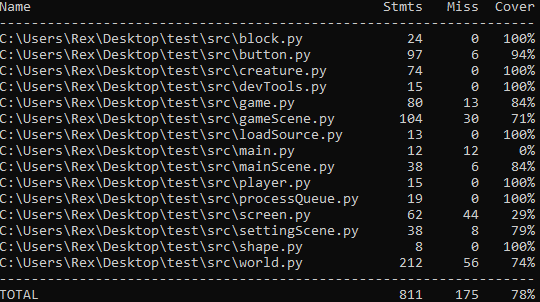
\includegraphics[scale=0.75]{coverage}
    \caption{\textbf{Code Coverage}}
\end{figure}
\FloatBarrier
\section{Appendix}

\subsection{Symbolic Parameters}

\begin{itemize}
    \item \textbf{AVG1: 7}
    \item \textbf{AVG2: 3}
    \item \textbf{LEARN\_MIN: 2}
    \item \textbf{LEARN\_MAX: 30}
    \item \textbf{RESPONSE: 0.1}
    \item \textbf{FALSE\_RESPONSE: 0.5}
    \item \textbf{OPERATION\_NUM: 10}
    \item \textbf{TIME: 60}
    \item \textbf{TRIES: 100}
\end{itemize}
\newpage
\begin{thebibliography}{9}
\bibitem{act} 
”Video Games and the law: Copyright, 
        Trademark and Intellectual Property”, NewMediaRights, 2020. [Online]. 
        Available: https://www.newmediarights.org/guide/legal/Video\_Games\_law\_
        Copyright\_Trademark\_Intellectual\_Property. [Accessed: 06- Feb- 
        2020].
\bibitem{mine} 
Fogleman, “fogleman/Minecraft,” 
        GitHub, 16-Feb-2019. [Online]. Available: 
        https://github.com/fogleman/Minecraft. [Accessed: 
        10-Feb-2020].

\end{thebibliography}
\end{document}